\documentclass[12pt,a5paper,landscape]{scrartcl}

\usepackage{vorschule}
\PassOptionsToPackage{dvipsnames}{xcolor}
\usepackage[
    typ=ohne,
%    fach=Mathematik,
    lerngruppe={0},
    nummer=1,
    module={Symbole,Lizenzen},
    seitenzahlen=keine,
    farbig,
    lizenz=cc-by-nc-sa-4,
]{schule}

\usepackage[
	typ=lerntheke,
	kuerzel=Ngb,
	reihe={Lernen mit Lerntheken},
	version={1.0 (2019-11-19)},
]{ngbschule}

\author{J. Neugebauer}
\title{Lerntheken}
\date{\Heute}

%\usepackage{pgfmorepages}
%\pgfmorepagesloadextralayouts
%\pgfpagesuselayout{4 on 2, odd then even}[a4paper]

\begin{document}

\begin{hilfekarte}{Die Lerntheke}{lerntheke}
	Anstatt alle zusammen im Klassenverbund zu lernen, arbeitet bei einer Lerntheke jeder in seinem eigenen Tempo an \textbf{Lernstationen}. Jede Lernstation besteht aus einer Karte, wie du sie gerade in der Hand hältst.

	\medskip
	\begin{wrapfigure}[7]{r}{0pt}
	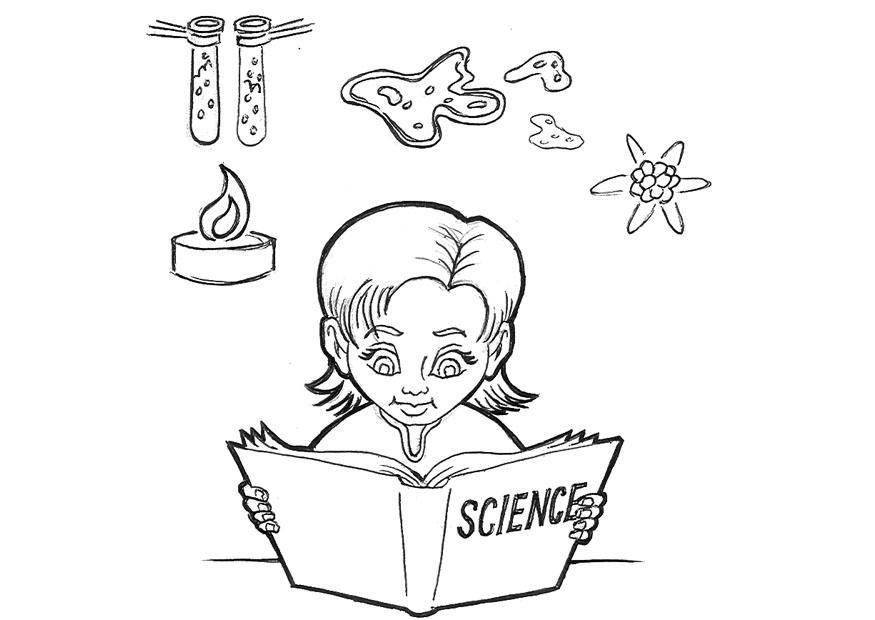
\includegraphics[width=5cm]{0.1-LT-Abb_Lernen}
	\end{wrapfigure}	
	Du entscheidest selber, welche Stationen du bearbeiten möchtest und wie. Aber denk daran, dass du am Ende trotzdem eine Klassenarbeit schreiben musst. Versuch also die Stationen in deinem Tempo zu bearbeiten, und nicht sofort die Lösungen abzuschreiben.
	
	\medskip
	Die Karten dieser Lerntheke zeigen dir, wie du an der Lerntheke arbeiten kannst, welche Hilfsmittel es gibt und wie die Stationenkarten aufgebaut sind.
	
	\medskip
	\begin{center}\large\bfseries
		Viel Spaß und Erfolg beim Lernen!
	\end{center}
	\infotext{\enquote{Malvorlage  Wissenschaft lernen} von \href{http://www.schulbilder.org}{Schulbilder.org}}
\end{hilfekarte}

\begin{loesungskarte}[Arbeitsweise]
\begin{center}
Hier findest du in der Regel die \textbf{Lösung einer Station}.
\end{center}

Zu Beginn erstellt du in deinem Heft eine Tabelle, in der du deinen Fortschritt festhältst. Die Tabelle enthält folgende Spalten:
%\begin{center}
%	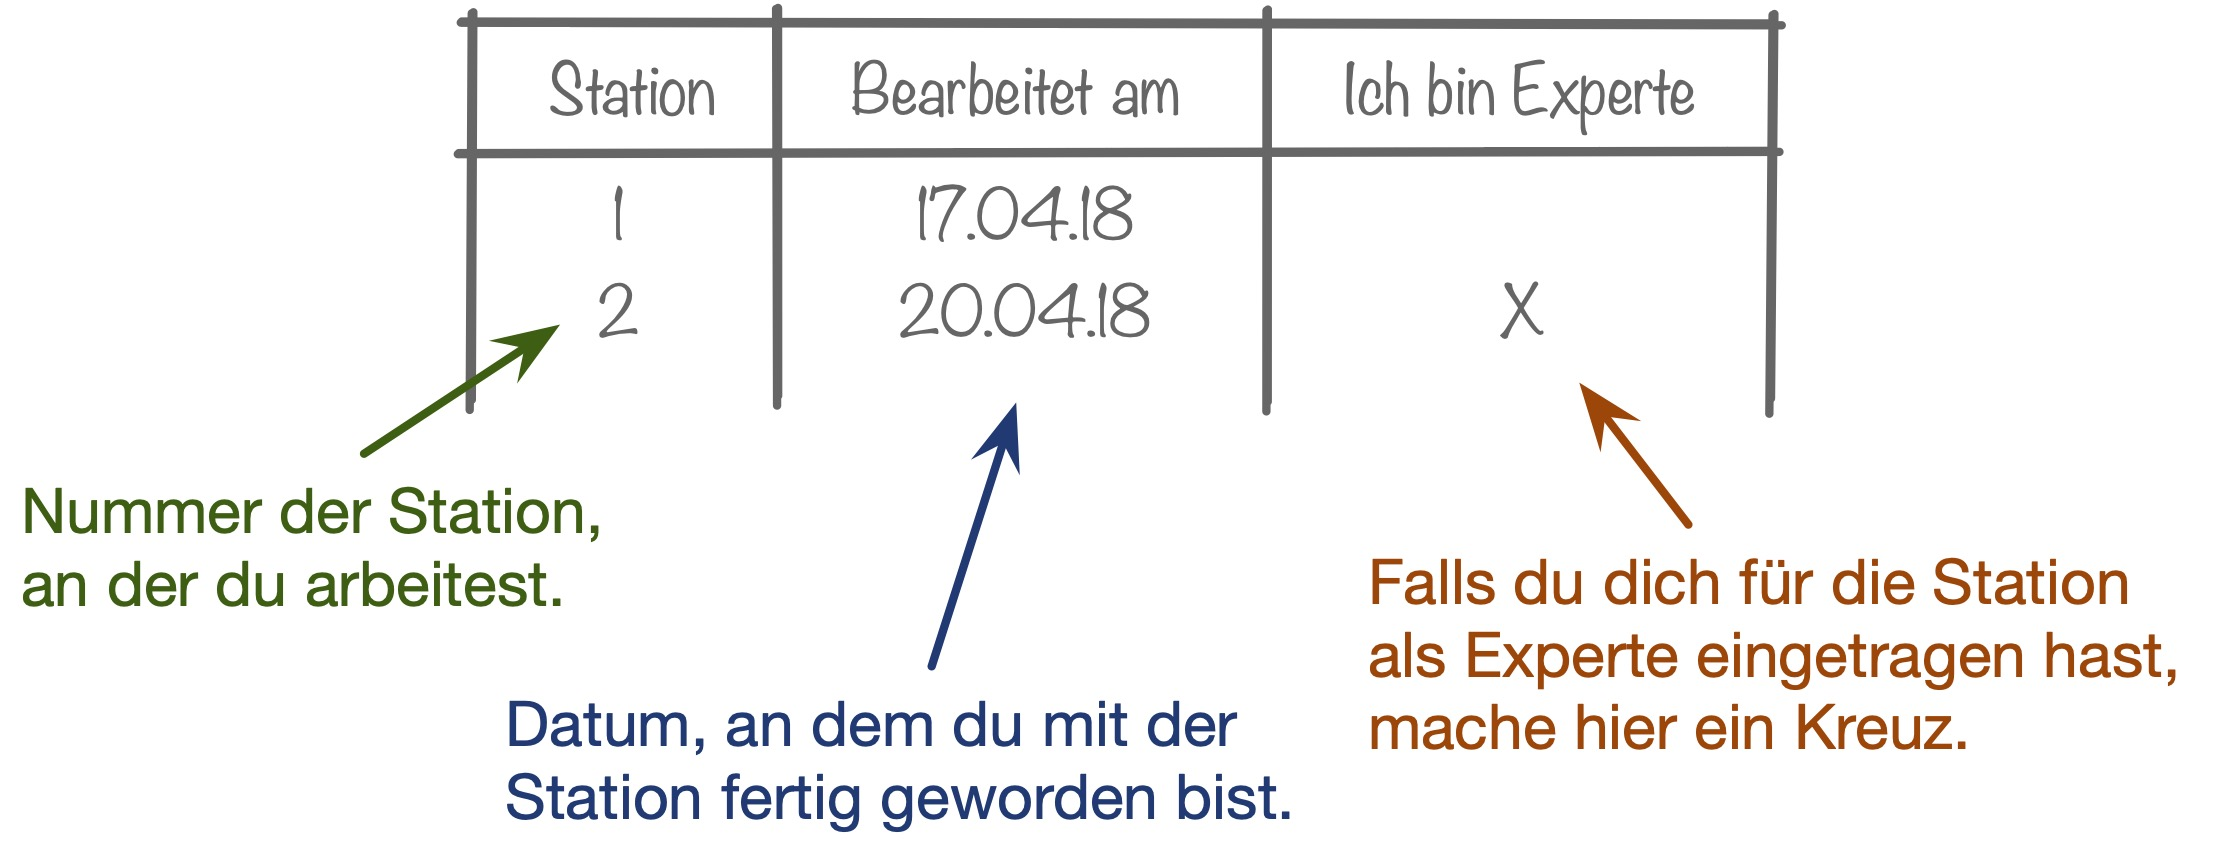
\includegraphics[width=\textwidth]{0.1-LT-Abb_Tabelle_2}
%\end{center}
	\begin{center}\scalebox{1}{
	\begin{tikzpicture}[]
		\node (tabelle) at (0,0) {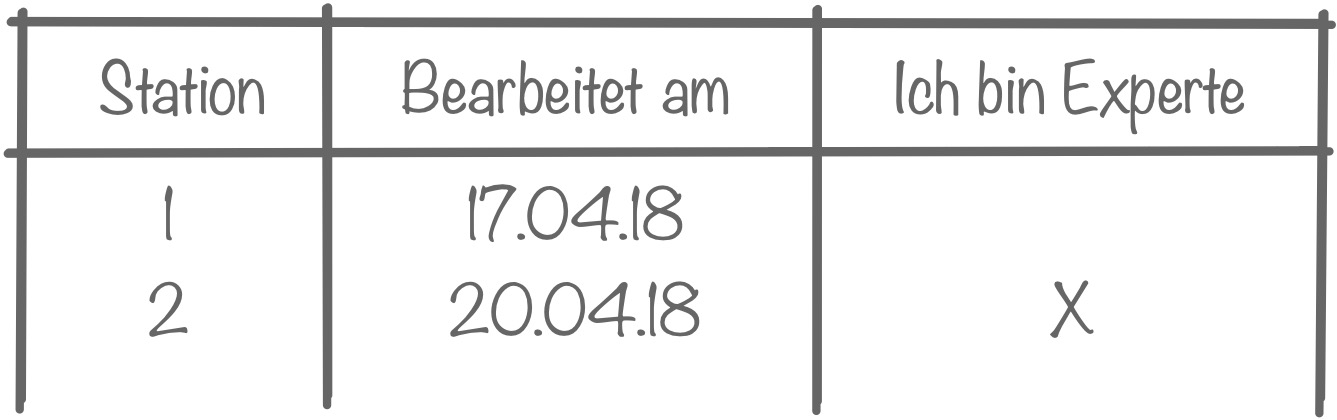
\includegraphics[width=10cm]{0.1-LT-Abb_Tabelle}};
		
		\node (marker1) at (-3.6,-1) {};
		\node (marker2) at (-.8,-1) {};
		\node (marker3) at (3,-1) {};
		
		\node[font=\color{blue!60!gray},text width=4cm,anchor=north] (text1) at (-6,-2) {Nummer der Station, an der du arbeitest.};
		\node[font=\color{green!50!black},text width=4cm,anchor=north] (text2) at (-1,-2.5) {Datum, an dem du mit der Station fertig geworden bist.};
		\node[font=\color{orange!80!black},text width=4cm,anchor=north] (text3) at (5,-2) {Falls du dich für die Station als Experte eingetragen hast, mache hier ein Kreuz.};
		
		\draw[draw=blue!60!gray,-latex,line width=2pt] (text1) -- (marker1);
		\draw[draw=green!50!black,-latex,line width=2pt] (text2) -- (marker2);
		\draw[draw=orange!80!black,-latex,line width=2pt] (text3) -- (marker3);
	\end{tikzpicture}}
	\end{center}
\end{loesungskarte}

\begin{hilfekarte}{Die Stationenkarten}{stationenkarten2}
	\begin{center}\scalebox{.9}{
	\begin{tikzpicture}[red color/.style={draw=red!80!black,line width=2pt},marker/.style={red color,fill=red!50!black,fill opacity=.2},red circle/.style={marker,circle,minimum width=1cm,minimum height=1cm},red rect/.style={marker},text field/.style={red color,fill=white,drop shadow,rounded corners=1pt,anchor=north west,font=\footnotesize},red line/.style={red color}]
		\node[draw=black] (karte) at (0,0) {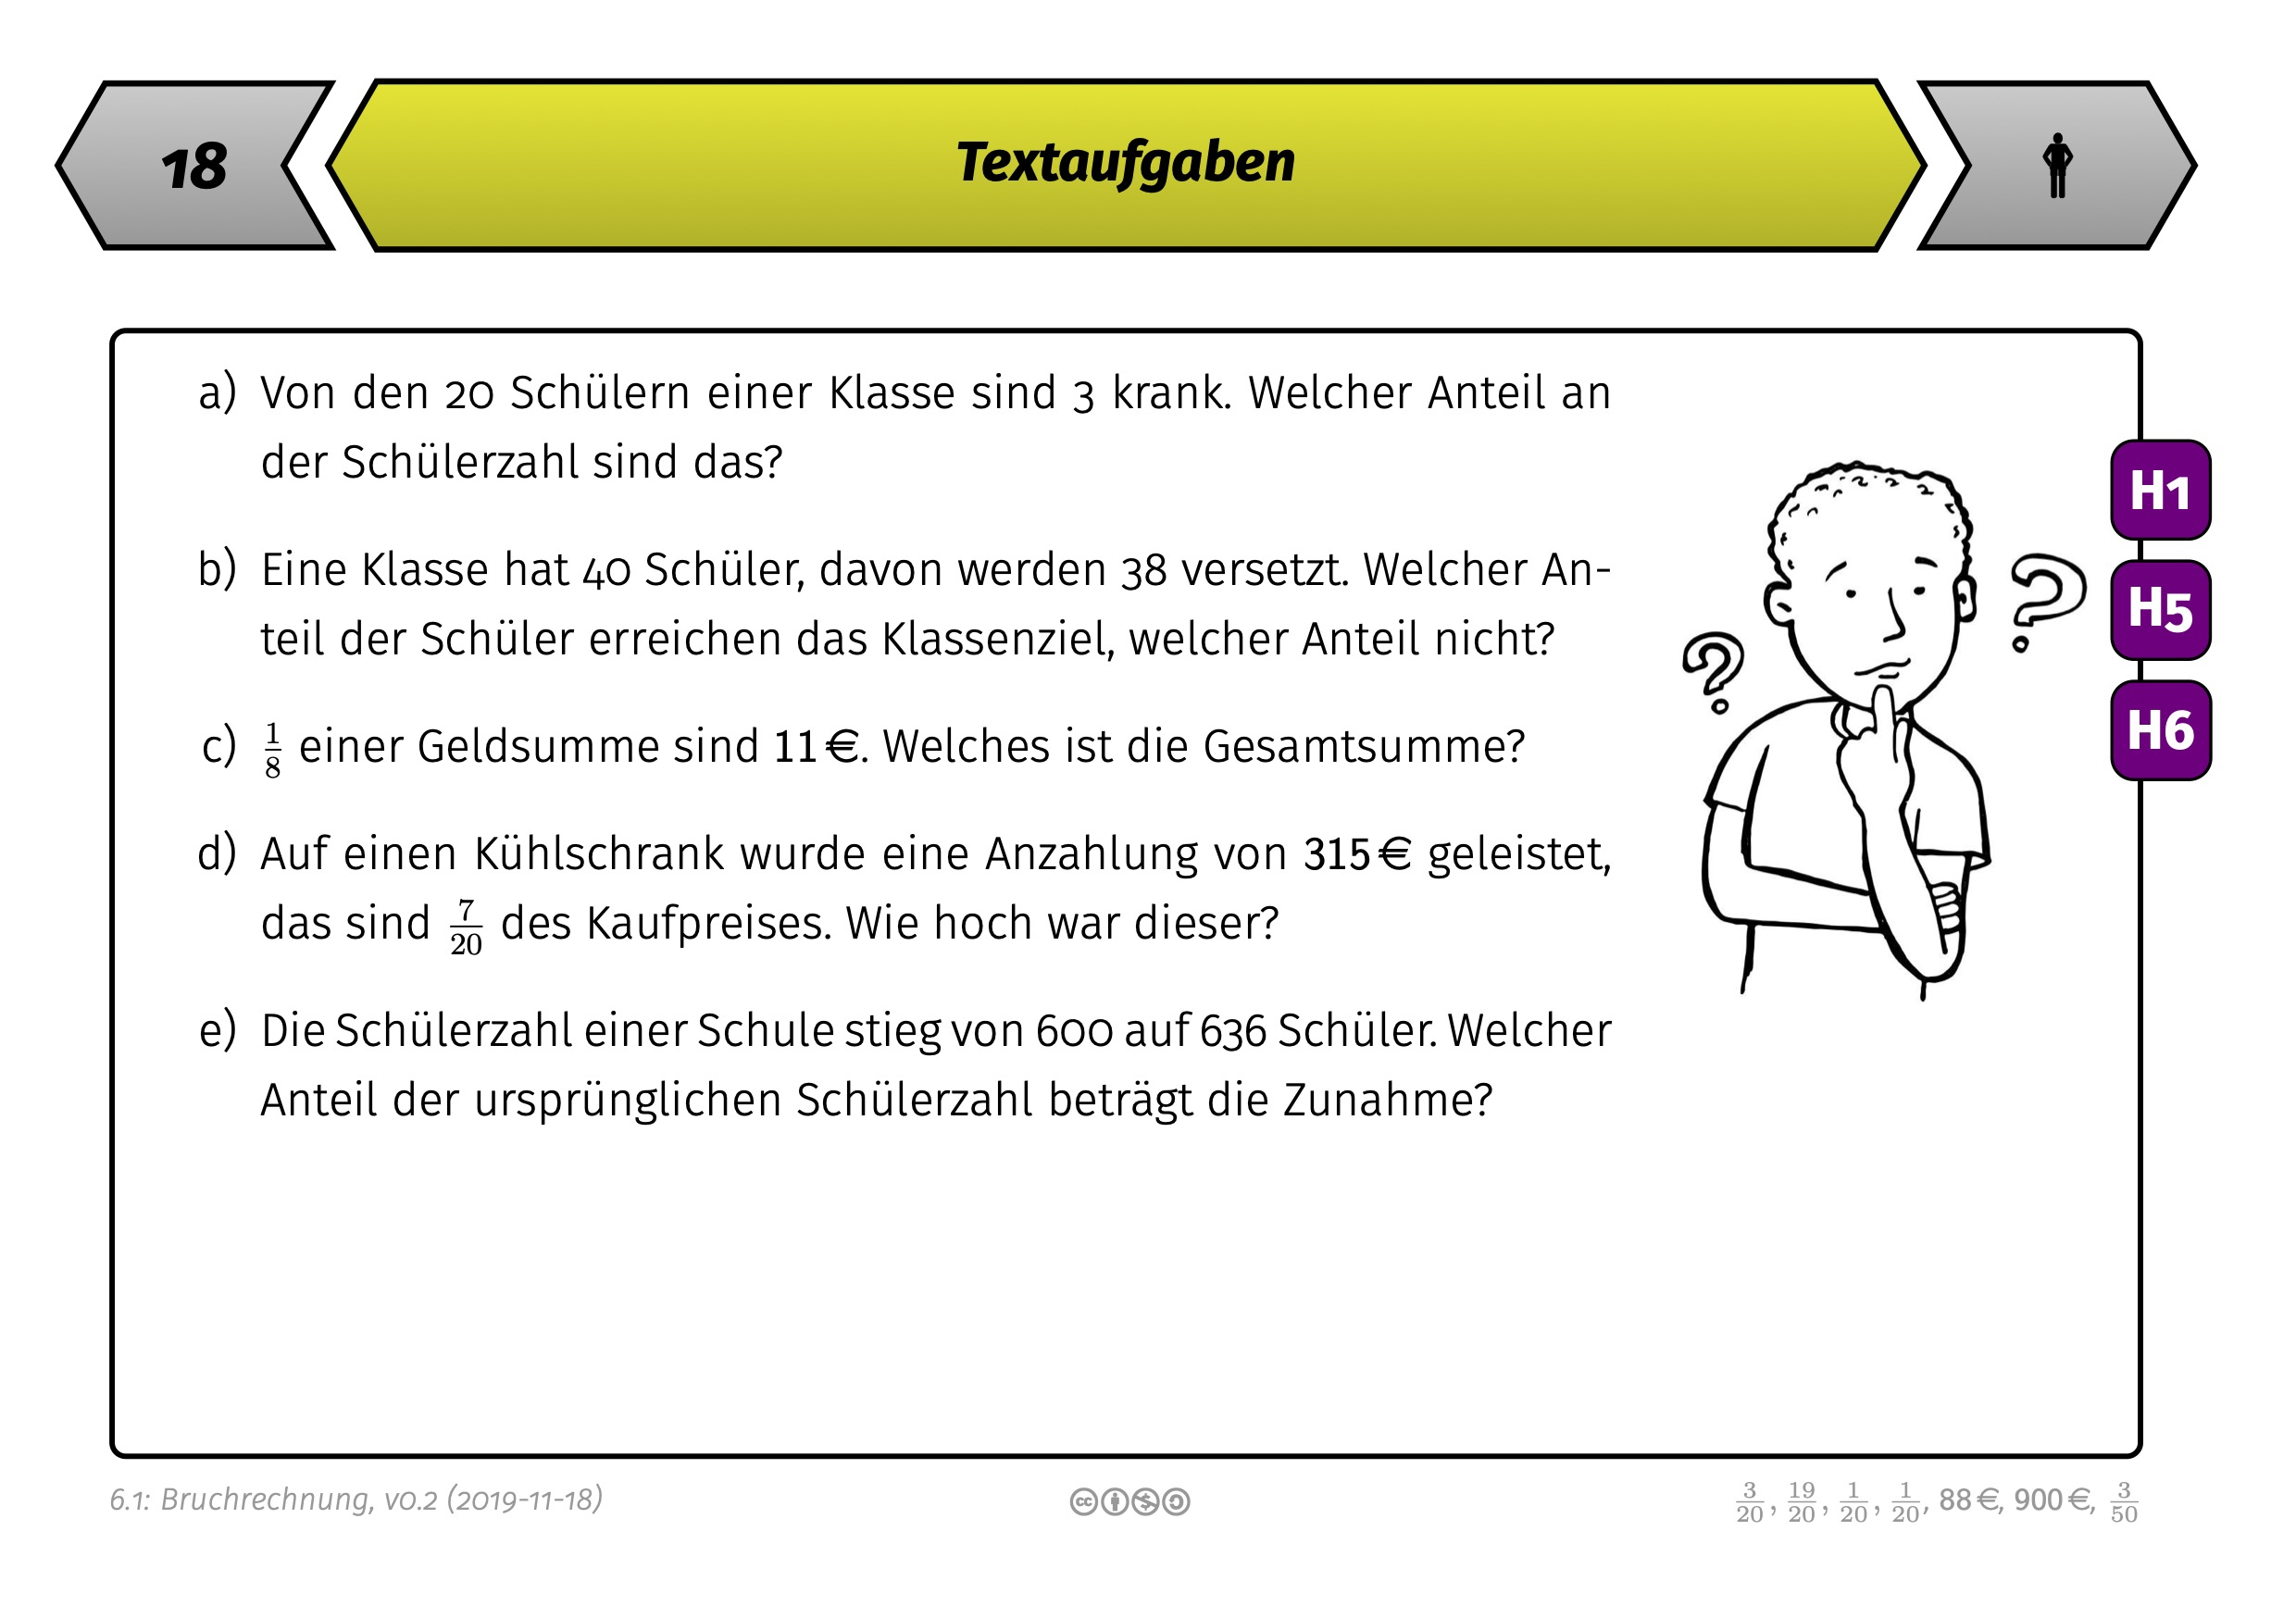
\includegraphics[width=8cm]{0.1-LT-Abb_Beispielkarte}};
		
		\node[red circle] (nrMarker) at (-3.3,2.25) {};
		\node[red circle] (symMarker) at (3.15,2.25) {};
		\node[red circle] (helpMarker) at (3.5,1.13) {};
		\node[red rect,minimum width=2cm,minimum height=.5cm] (infoMarker) at (2.8,-2.4) {};
		\node (taskMarker) at (-1.5,-1.4) {};
		\node (headMarker) at (0,2.4) {};
		
		\node[text field,text width=11cm] (headText) at (-8,5.6) {Die Farbe der Kopfzeile zeigt die \textbf{Stufe} der Station an:\\
		\textcolor{green!80!black}{Grün: Grundlagen lernen}\\
		\textcolor{orange!80!black}{Gelb: Anwendung der Grundlagen}\\
		\textcolor{red!80!black}{Rot: Komplexe Aufgaben, die mehrere Grundlagen verknüpfen}};
		
		\node[text field,text width=4cm] (nrText) at (-9.2,3) {Jede Station hat eine \textbf{Nummer}. Die Stationen können, \emph{müssen aber nicht} in dieser Reihenfolge bearbeitet werden. Überleg dir am besten eine \emph{eigene Reihenfolge}.};
		
		\node[text field,text width=3cm] (symText) at (4.5,5.2) {{\normalsize\symEinzel} Einzelarbeit\\
		{\normalsize\symPartner} Partnerarbeit\\
		{\normalsize\symGruppe} Gruppenarbeit};
		
		\node[text field,text width=3cm] (helpText) at (4.9,2.7) {Diese Symbole zeigen dir an, auf welchen \textbf{Hilfekarten} du bei Problemen nachsehen kannst.};
		
		\node[text field,text width=4cm] (infoText) at (4.5,-1.4) {Hier stehen manchmal klein die \textbf{Lösungen} zur Karte, anstatt auf der Rückseite. Oder hier stehen Informationen zu den verwendeten Bildern.};
		
		\node[text field,text width=4cm] (taskText) at (-8.8,-1) {Das wichtigste jeder Station sind die \textbf{Aufgaben}. Lies sie \emph{sorgfältig} und bearbeite sie \emph{möglichst eigenständig}. Zur Kontrolle findest du auf der Rückseite die Lösung.};
		
		
		\draw[red line] (nrText) -- (nrMarker);
		\draw[red line] (symText) -- (symMarker);
		\draw[red line] (helpText) -- (helpMarker);
		\draw[red line] (infoText) -- (infoMarker);
		\draw[red line,-latex] (taskText) -- (taskMarker);
		\draw[red line,-latex] (headText) -- (headMarker);
	\end{tikzpicture}}
	\end{center}
\end{hilfekarte}

\begin{loesungskarte}
\begin{center}
Hier findest du in der Regel die \textbf{Lösung einer Station}.
\end{center}

Bei manchen Stationen ist die Lösung aber auch \emph{klein auf die Vorderseite gedruckt}, oder ist zum Beispiel als \emph{Kontrollwort in der Aufgabe} angegeben.

\bigskip
Du solltest dich bemühen die Stationen möglichst \emph{eigenständig} zu lösen. Hast du Probleme, kannst du zunächst die \emph{Hilfekarten} (siehe \ref{hilfe:hilfekarten}) zu Rate ziehen. Danach kannst du auf dem Expertenposter (siehe \ref{hilfe:expertenposter}) nachsehen, ob dir vielleicht schon jemand bei der Station helfen kann. Bist du immer noch unsicher, dann kann dir der Lehrer (siehe \ref{hilfe:lehrer}) bestimmt weiterhelfen.
\end{loesungskarte}

\begin{hilfekarte}{Hilfekarten}{hilfekarten}
Hilfekarten erkennst du an der \textcolor{violet}{violetten Kopfzeile}. Die Nummern der Hilfekarten beginnen mit einem \enquote{H} (z.B. H1, H2, ...).

\begin{center}\begin{tikzpicture}[scale=.6]
	\node[header,help,minimum width=.5\textwidth] (header2) {Addition von Brüchen};
	\node[left side,left=of header2,xshift=.5cm,minimum width=2cm,label={[side label left]center:H2}] (left2) {};
	\node[right side,right=of header2,xshift=-.5cm,minimum width=2cm,label={[side label right]center:\Kartensymbol}] (right2) {};
\end{tikzpicture}\end{center}

Die Nummern der Hilfekarten, die du für deine Station nutzen kannst, findest du in den \textcolor{violet}{violetten Symbolen} am rechten Rand der Stationskarte.

\begin{center}
	\begin{tikzpicture}
		\draw (0,-1) -- (0,1);
		\node at (0,0) [help mark] {H2};
	\end{tikzpicture}
\end{center}
\end{hilfekarte}


\begin{loesungskarte}[Rückseiten]
Auf der \emph{Rückseite} einer Karte findest du in der Regel die \emph{Lösungen} der Aufgaben.

\medskip
Hilfekarten haben normalerweise keine Lösung. Aber wenn auf der Vorderseite nicht genug Platz war, stehen auf der Rückseite manchmal weitere Informationen.

\medskip
So wie hier. \symSmileyZwinkernd
\end{loesungskarte}

\begin{hilfekarte}{Das Expertenposter}{expertenposter}
Hast du eine Station bearbeitet und \emph{fühlst dich so sicher} dabei, dass du anderen Schülerinnen und Schülern die Lösung \emph{erklären} kannst, \begin{wrapfigure}[6]{r}{0pt}
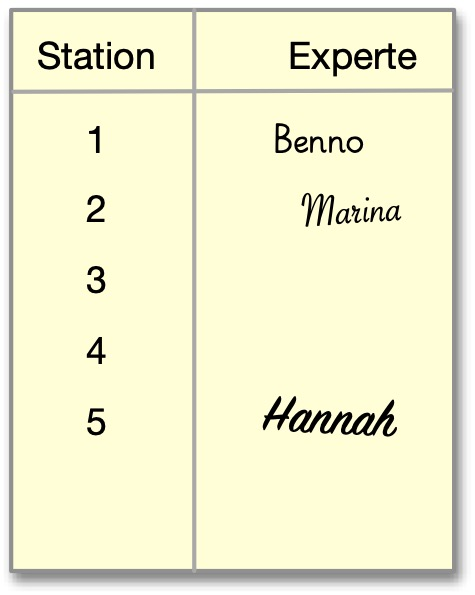
\includegraphics[width=4.5cm]{0.1-LT-Abb_Expertenposter}
\end{wrapfigure}dann trag dich auf dem Expertenposter als \emph{Experte oder Expertin} ein.

\medskip
Zu jeder Station kann es zwei Experten geben.

\bigskip
Kommst du bei einer Station nicht weiter, und helfen dir die Hilfekarten auch nicht, dann guck auf dem Expertenposter nach, ob es schon einen Experten oder eine Expertin für die Station gibt. Frag denjenigen oder diejenige nach Hilfe.
\end{hilfekarte}

\leereKarte

\begin{hilfekarte}{Der Lehrer}{lehrer}
Haben dir die Hilfekarten und die Experten / Expertinnen zu deiner Station nicht weitergeholfen (oder falls es keine Hilfen oder Expertinnen gibt), dann kannst du natürlich auch den Lehrer um Hilfe bitten.

\medskip
\begin{wrapfigure}[7]{l}{0pt}
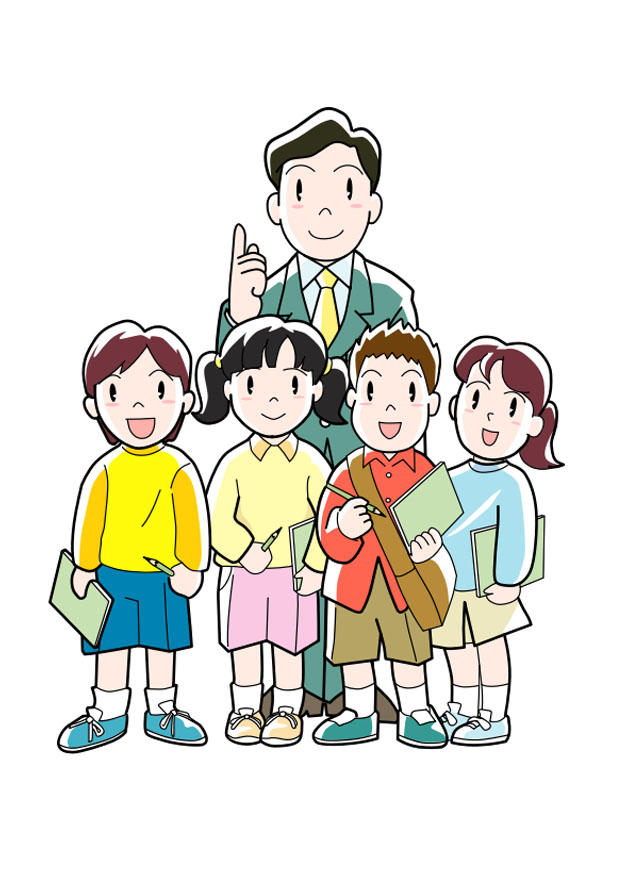
\includegraphics[width=4cm]{0.1-LT-Abb_Lehrer}
\end{wrapfigure}
Aber am meisten lernt man, wenn man \emph{erstmal selber versucht}, eine Station zu lösen. \emph{Also denk zunächst gut nach, wie du vorgehen kannst, bevor du zum Lehrer kommst.} Bestimmt kommt dir dabei schon eine gute Idee für die Lösung.

\medskip
Hast du eine Station gelöst kannst du dein Ergebnis mit den \emph{Lösungen auf der Rückseite} überprüfen. Hast du dann noch Fragen beantwortet sie dir der Lehrer gerne.
\infotext{\enquote{Malvorlage  Lehrer und Schüler} von \href{http://www.schulbilder.org}{Schulbilder.org}}
\end{hilfekarte}

\leereKarte
	
\end{document}